\documentclass{article}
% --- watermark (auto-inserted) ---
\usepackage{xcolor}
\usepackage{xfp}% \fpeval; in the kernel since 2022, harmless on older LaTeX
\usepackage{draftwatermark}
\newlength{\watermarkTextWidth}
\AddToHook{begindocument/end}{%
  \SetWatermarkText{\normalfont Generated by The Agentic Scientist}%
  \SetWatermarkFontSize{10pt}%
  \SetWatermarkLightness{0.85}%
  \settowidth{\watermarkTextWidth}{\normalfont\fontsize{10pt}{12pt}\selectfont Generated by The Agentic Scientist}%
  \edef\watermarkScale{\fpeval{0.8 * sqrt(\paperwidth**2 + \paperheight**2) / \watermarkTextWidth}}%
  \edef\watermarkAngle{\fpeval{atand(\paperheight/\paperwidth)}}%
  \SetWatermarkScale{\watermarkScale}%
  \SetWatermarkAngle{\watermarkAngle}%
}
% --- end watermark ---
 % For LaTeX2e
\usepackage{paper,times}

\usepackage{hyperref}
\usepackage{url}
\usepackage{graphicx}
\usepackage{booktabs}
\usepackage{amsmath,amssymb}
\usepackage{subcaption}

\newcommand{\nrmse}{\mathrm{nRMSE}}

\title{How Far Do $k$ Benchmarks Go? Cold-Start Benchmark Selection and Score Imputation on Family-Disjoint Held-Out Models}

\begin{document}
\maketitle

\begin{abstract}
Evaluating a new model on every benchmark of a leaderboard is expensive, yet benchmarks may be substantially redundant, so a few runs might carry information about the rest. We study the cold-start version of this problem: given a model$\times$benchmark history with missing cells, commit to $k$ benchmarks before seeing the new model, run only those, and impute the rest. We evaluate a family of selector--imputer pairs built from a rank-Gauss transform, an EM-fitted Gaussian with missing data, cross-validated wrapper selection, and a per-target non-negative stack of imputers; the identity of the exact source tree evaluated in the sealed run is not established by the retained artifacts, and we presume it is the development-selected pair or its latent-skill extension. Evaluation uses held-out models from model families disjoint from the history on three public leaderboards (MTEB, Open LLM Leaderboard, HELM Lite). The evaluated pair attains pooled normalized RMSE 0.562, a mean relative error reduction (skill) of 0.434 against column-mean imputation, and beats permuted-observation controls by a wide margin, but its skill over random-$k$ selection with a ridge imputer is only 0.016. On MTEB the error falls from 0.787 at $k{=}2$ to 0.638 at $k{=}20$ with sharply diminishing returns. Selector and imputer are scored jointly, three seeds do not resample held-out models, and no component ablation was run, so we do not attribute the gain to either part.
\end{abstract}

\section{Introduction}
A full evaluation of a language or embedding model touches dozens to hundreds of benchmarks, each costing compute, time and human effort. Public leaderboards meanwhile accumulate large model$\times$benchmark score matrices, and benchmark suites such as MMLU, BIG-bench, HELM and MTEB \citep{Hendrycks2021MMLU,Srivastava2023BIGbench,Liang2023HELM,Muennighoff2023MTEB} are plausibly overlapping in what they measure: agreement analyses across benchmarks and low-dimensional capability models fitted to public evaluations both bear on how related benchmark scores are \citep{Perlitz2024BenchBench,Ruan2024ObservationalScaling,Polo2024Sloth}. This suggests a budgeted-evaluation protocol: an evaluator holding a historical matrix with $M$ models, $N$ benchmarks and missing cells receives a new model, can afford only $k\ll N$ benchmark runs, and wants to infer the scores on the other $N-k$ benchmarks as accurately as possible. Two decisions then matter: \emph{which} $k$ benchmarks to run, and \emph{how} to turn their scores into predictions. A practitioner also needs to know how large $k$ must be.

Prior work on cheaper evaluation mostly reduces the number of \emph{items} within one benchmark \citep{Polo2024TinyBenchmarks,Vivek2024AnchorPoints,Perlitz2024EfficientBenchmarking}, distills a handful of benchmarks into a sparse one \citep{Kipnis2024Metabench}, or fits low-dimensional capability models across many benchmarks \citep{Ruan2024ObservationalScaling,Polo2024Sloth}. The setting studied here differs in three ways: the selection is committed \emph{before} any score of the new model is seen, the target is the score on every unrun benchmark, and the new model comes from a family that is absent from the history.

\paragraph{Research question and hypotheses.} When only $k$ benchmarks can be run on a new model, how accurately can a history-fitted selector--imputer pair recover its other scores, how does the error fall with $k$, and how much of the gain comes from cross-benchmark structure versus the choice of which $k$ to run? We examine four hypotheses.
\textbf{H1}: observed scores on a selected subset predict the remaining scores better than history-only column means.
\textbf{H2}: the error decreases with $k$ with diminishing returns.
\textbf{H3}: a model-based selector adds accuracy beyond random selection under a comparable imputer.
\textbf{H4}: difficulty differs across leaderboards.

\paragraph{What the evidence supports.} Using a sealed evaluation on family-disjoint held-out models from three leaderboards, H1 and H2 are supported, H4 is observed but confounded by the number of benchmarks per leaderboard, and H3 is not tested by the sealed evaluation, because selector and imputer are scored jointly; the 0.016 skill margin over random-$k$ ridge is small and unresolved. Figure~\ref{fig:overview} summarises the protocol.

\paragraph{Contributions.}
(i) A precise cold-start protocol with committed selection, family-disjoint held-out models, evaluator-owned baselines and negative controls, and a hierarchical aggregation rule (Section~\ref{sec:protocol}).
(ii) A reimplementable selector--imputer design built from standard components: rank-Gauss transform, EM Gaussian, wrapper selection, NNLS stacking (Section~\ref{sec:method}).
(iii) An error-versus-$k$ curve on MTEB and per-leaderboard errors, with skill relative to three baselines and a permutation control (Section~\ref{sec:results}).
(iv) A calibrated account of what the evidence cannot show: no ablation, no theory check, joint scoring of selector and imputer, and seed variation that does not reflect held-out sampling (Section~\ref{sec:limits}).

\begin{figure}[t]
\centering
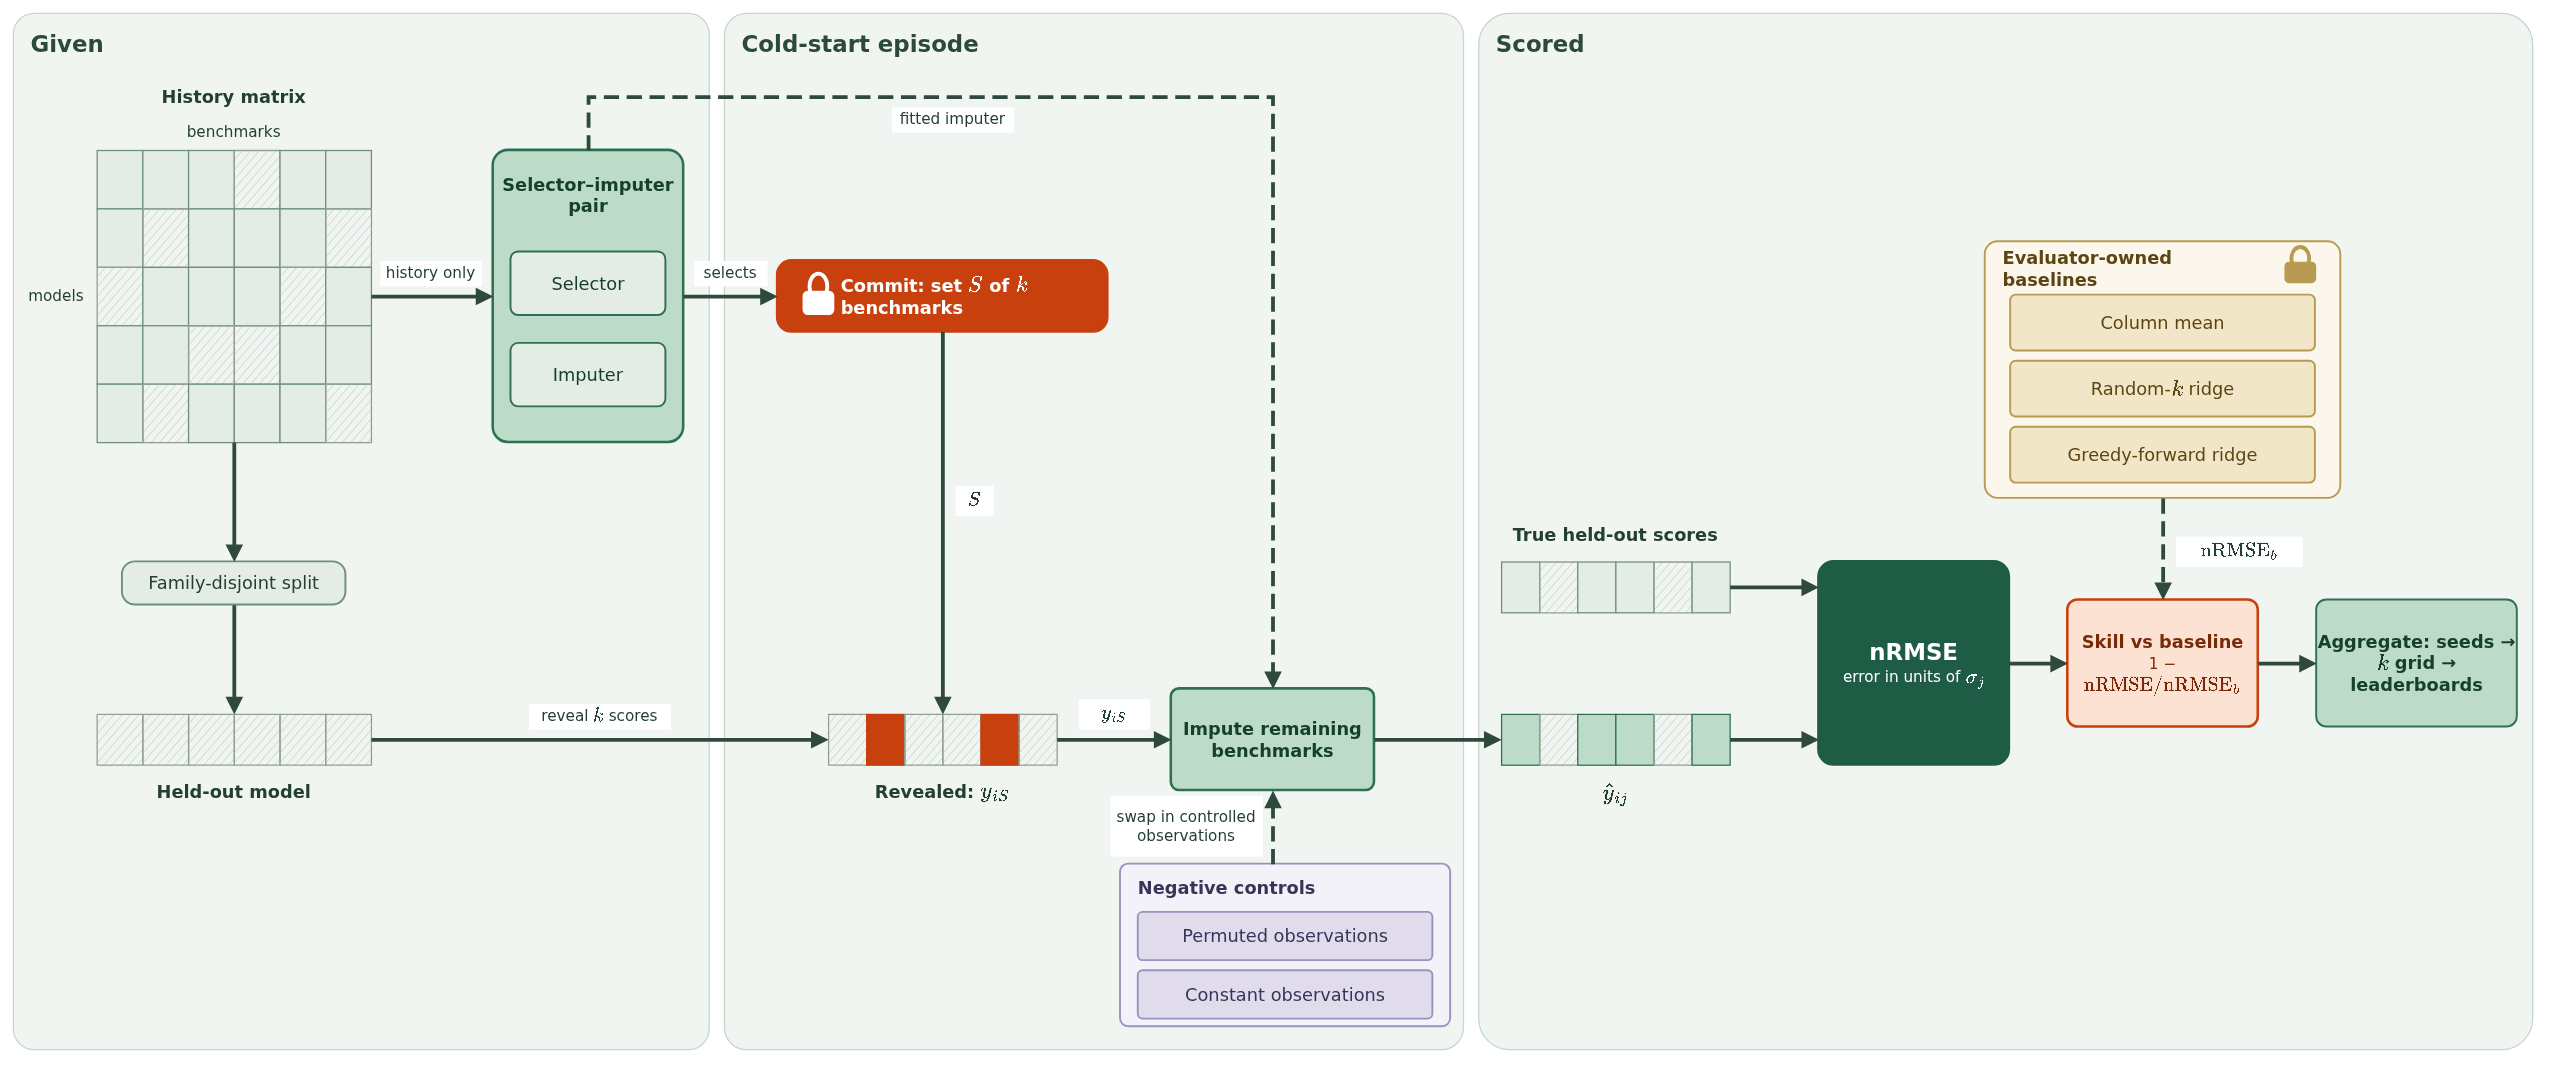
\includegraphics[width=\textwidth]{figures/protocol_overview.png}
\caption{Cold-start protocol. A history matrix with missing cells is given to the method; it commits to $k$ benchmark indices; only the new model's scores on those $k$ benchmarks are revealed; the method predicts all other benchmarks; error is measured in units of history column standard deviations and compared with column-mean, random-$k$ ridge and greedy-forward ridge baselines and with permuted-observation controls.}
\label{fig:overview}
\end{figure}

\section{Related Work}
\paragraph{Benchmark suites and their overlap.} Multi-task suites aggregate many sub-benchmarks \citep{Hendrycks2021MMLU,Srivastava2023BIGbench,Liang2023HELM,Muennighoff2023MTEB}. Agreement analyses across benchmarks \citep{Perlitz2024BenchBench} bear on how related benchmark scores are; here the target, the held-out split and the aggregation are defined explicitly.

\paragraph{Cheaper evaluation within or across benchmarks.} tinyBenchmarks, anchor points and efficient-benchmarking studies shrink the number of items of a single benchmark while preserving its score or ranking \citep{Polo2024TinyBenchmarks,Vivek2024AnchorPoints,Perlitz2024EfficientBenchmarking}. metabench distills a sparse benchmark from several benchmarks \citep{Kipnis2024Metabench}. Fluid benchmarking goes further by choosing items adaptively under an item-response model of latent ability \citep{Hofmann2025Fluid}. These works reduce or adapt item counts within a benchmark or a fixed suite; here the unit of selection is a whole benchmark, the choice is committed before any score of the new model is seen, and the target is every benchmark not run.

\paragraph{Latent-capability and scaling views.} Observational scaling laws and skill scaling laws explain multi-benchmark performance through a few latent capability factors estimated from public evaluations \citep{Ruan2024ObservationalScaling,Polo2024Sloth}, and item response theory has long modelled responses through latent ability \citep{Embretson2000IRT}. These latent-factor predictors are the closest benchmark-level relatives of the present setting; we did not run them as baselines, so how they compare under our protocol is left open. Our imputer uses a Gaussian dependence structure rather than an explicit latent-factor law, and we evaluate on family-disjoint models rather than within-family extrapolation.

\paragraph{Missing data, matrix completion and design.} Gaussian models with missing entries are fitted by EM \citep{Dempster1977EM} under missingness assumptions discussed by \citet{Rubin1976Inference}. Low-rank and probabilistic matrix completion \citep{Candes2009MatrixCompletion,Salakhutdinov2007PMF} are the standard alternatives for filling score matrices. Selecting observations to minimise posterior uncertainty is an experimental-design problem \citep{Chaloner1995BayesianDesign}; for Gaussian processes, greedy selection of informative variables has near-optimality guarantees when the objective is submodular \citep{Nemhauser1978Submodular,Krause2008NearOptimalSensor}. Stacked generalization combines predictors with weights fitted on held-out predictions \citep{Wolpert1992Stacked,Breiman1996Stacked}, and ridge regression \citep{Hoerl1970Ridge} is the linear baseline used by the evaluator.

\section{Method}\label{sec:method}

\subsection{Problem setup and success criterion}\label{sec:setup}
Let $X\in\mathbb{R}^{M\times N}$ be a history matrix with observation mask $O\in\{0,1\}^{M\times N}$; benchmark $j$ has history mean $m_j$ and standard deviation $\sigma_j$ computed over its observed cells. A new model $i$ has scores $y_{ij}$ on a subset $\mathcal{O}_i$ of benchmarks (not every model was run on every benchmark). A method must (a) output a set $S$ of $k$ benchmark indices \emph{before} seeing any new-model score (non-adaptive selection), and (b) given $y_{iS}$ (only the entries in $\mathcal{O}_i\cap S$), output predictions $\hat y_{ij}$ for all $j$. Scoring uses the cells $\mathcal{C}_i=\mathcal{O}_i\setminus S$. For one evaluation episode with $T$ held-out models,
\begin{equation}
\nrmse=\sqrt{\frac1T\sum_{i=1}^{T}\frac{1}{|\mathcal{C}_i|}\sum_{j\in\mathcal{C}_i}\Big(\frac{\hat y_{ij}-y_{ij}}{\sigma_j}\Big)^2},
\end{equation}
so every held-out model has equal weight and every benchmark is on the scale of its history spread. A baseline $b$ yields the skill
\begin{equation}
\mathrm{skill}_b = \mathrm{clip}\big(1-\nrmse/\nrmse_b,\,-1,\,1\big),
\end{equation}
the relative error reduction against that baseline, which is $0$ at parity and negative when worse.

\subsection{Design rationale}\label{sec:rationale}
If benchmark scores are jointly Gaussian with covariance $\Sigma$ and benchmarks in $S$ are observed, the conditional mean $\mathbb{E}[y_U\mid y_S]$ ($U$ the unrun benchmarks) minimises mean squared error, and the expected squared error summed over $U$ equals $\operatorname{tr}\Sigma_{U\mid S}$. Choosing $S$ greedily to reduce this trace (an A-optimal design) is therefore a principled selector \emph{under the Gaussian model}. Concretely, for a row-vector of scores $y\sim\mathcal{N}(\mu,\Sigma)$ and observation noise $\lambda\ge 0$, the posterior covariance after observing benchmark $j$ is $R'=R-R_{\cdot j}R_{j\cdot}/(R_{jj}+\lambda)$ with $R$ initialised at $\Sigma$, and the resulting drop of the summed variance over the remaining benchmarks is $\sum_{i\in U,\,i\neq j}R_{ij}^2/(R_{jj}+\lambda)$. A benchmark scores highly if it is strongly correlated with many others and itself has substantial variance, so redundant benchmarks are avoided once one of them has been chosen, because the update deflates their shared variance. The classical near-optimality guarantees for greedy selection \citep{Nemhauser1978Submodular,Krause2008NearOptimalSensor} apply to submodular objectives; we do not claim that the trace criterion with noise and missing data satisfies the required conditions here. We state the Gaussian argument only as motivation: we did not check it against a controlled experiment, and real score matrices are bounded, skewed and sparsely observed, which can make the trace criterion misaligned with realised held-out error. Three design choices address this misalignment:
(1) a per-benchmark rank-Gauss transform makes marginals closer to normal, with predictions mapped back through the stored history quantiles and clipped to the observed history range;
(2) a wrapper selector scores candidate benchmarks directly by cross-validated held-out-model error, instead of the model-based trace alone;
(3) a per-target non-negative-least-squares stack \citep{Lawson1995NNLS,Breiman1996Stacked} lets each target benchmark weight several imputers (Gaussian conditional means, ridge, nearest-neighbour models, column median), with a median-shrinkage fallback when the stack does not beat the median in cross-validation.
All tuning uses history models only.

\subsection{Compared approaches}\label{sec:variants}
\textbf{Proposed pair.} The selector--imputer pair of Section~\ref{sec:impl}, selected on the development partition as the best-scoring configuration. The sealed evaluation presumably ran this pair or its latent-skill extension (below), which have identical development scores; no artifact records which source tree was evaluated, so this identity is not established. Statements about the ``evaluated pair'' therefore refer to this selector--imputer family. \textbf{Variant under search.} A simpler pair: z-scored columns, EM Gaussian, covariance-trace greedy selection with a coverage weighting, and the ridge-regularised Gaussian conditional mean, with shrinkage, factor rank and ridge strength tuned by history cross-validation. A third pair adds a monotone-link latent-skill member to the stack and a latent A-optimal selector candidate. The proposed pair and the simpler pair differ in several components at once (transform, selector candidates, stack, clipping), so their comparison (Table~\ref{tab:search}) is a comparison of configurations, not an ablation. \textbf{Evaluator baselines.} (a) \emph{Column mean}: predict each benchmark's history mean. (b) \emph{Random-$k$ ridge}: five random $k$-subsets (seeded from the dataset, $k$ and draw index), ridge imputer fitted on a rank-5 SVD-completed history (40 completion iterations), ridge strength chosen by leave-one-out over four values; the mean $\nrmse$ over draws is the baseline. (c) \emph{Greedy-forward ridge}: forward selection (up to 20 benchmarks) minimising leave-one-out ridge error on the remaining benchmarks of the completed history, with the same ridge imputer. Both ridge baselines share their imputer, so they probe selection with the imputer fixed; the proposed pair changes both selector and imputer.

\subsection{Selector and imputer}\label{sec:impl}
The constants and routines below are read from the proposed-pair source copy; the identity of the sealed-evaluated source tree is not established (presumably this pair or its latent-skill extension, Section~\ref{sec:variants}).

\paragraph{Representation and EM.} Two representations of the history are built: z-scoring (clipped at $\pm8$) and an empirical rank-Gauss map $\Phi^{-1}\big((r-\tfrac12)/n\big)$ per benchmark (average ranks; benchmarks with fewer than eight observations or four distinct values fall back to z-scores). For each, EM fits $\mathcal{N}(\mu,\Sigma)$ with missing entries, applying diagonal shrinkage $\Sigma\leftarrow(1-\epsilon)\Sigma+\epsilon\,\mathrm{diag}(\Sigma)$ ($\epsilon=0.02$) in each M-step (at most 60 iterations, tolerance $10^{-4}$, 25-s budget).

\paragraph{Selection.} Candidate subsets come from (i) covariance-trace greedy A-optimal selection: with $R$ the current posterior covariance, add $j$ maximising $\sum_{i\in U,i\ne j}R_{ij}^2/(R_{jj}+\lambda)$, then update $R\leftarrow R-R_{\cdot j}R_{j\cdot}/(R_{jj}+\lambda)$; and (ii) a greedy forward \emph{wrapper} that adds the benchmark minimising five-fold held-out-model squared error of the conditional-Gaussian predictor, with all candidates scored by batched matrix products and an optional coverage weighting (benchmarks missing for many history models are less informative). For each representation and candidate rule, the subset with the lowest history cross-validation error in raw benchmark units is chosen (up to 250 candidates per step).

\paragraph{Imputation.} For a new model, the Gaussian conditional mean $\mu+\Sigma_{\cdot S}(\Sigma_{SS}+\lambda I)^{-1}(y_S-\mu_S)$ conditions only on the selected benchmarks that model actually has. Shrinkage, factor rank and $\lambda$ are tuned by five-fold history cross-validation. The stack uses, per target benchmark, non-negative weights over six base predictors (three Gaussian conditional means at shrinkage 0, 0.15 and 0.3, ridge on the selected benchmarks, and kNN with 5 and 15 neighbours) plus an implicit column-median term, fitted on out-of-fold history predictions and regularised toward a pooled weight vector; a regularisation strength is chosen from six values by cross-validation. Outputs are mapped back to raw units, clipped to the history range, and replaced by the observed value for selected benchmarks; a model with no selected score receives the column median.

\paragraph{Cost and applicability.} All components are CPU-only NumPy. Fitting plus selection for one $(\text{dataset},k)$ episode is dominated by EM and cross-validation; the sealed evaluation of 14 episodes per seed took about 157--161 seconds per seed. The method presumes a history matrix with enough coverage per benchmark and a new model whose scores are exchangeable with history models after transformation, which family-disjoint evaluation tests but does not guarantee. In the proposed-pair source copy, which is not verified as the sealed-evaluated tree, wall-clock guards skip optional selector candidates after 70 s, fall back to a smaller tuning grid after 150 s, and skip stacking (leaving the Gaussian-only model) after 210 s; the timing above is a property of the sealed run and may not transfer to that copy.

\subsection{Experimental protocol}\label{sec:protocol}
\paragraph{Data.} Sealed evaluation uses three public leaderboards at pinned revisions: MTEB results (297 benchmark columns; 124 history and 37 held-out models), the Open LLM Leaderboard table (six benchmarks, namely IFEval \citep{Zhou2023IFEval}, BBH \citep{Suzgun2023BBH}, MATH Level~5 \citep{Hendrycks2021MATH}, GPQA \citep{Rein2023GPQA}, MuSR \citep{Sprague2023MuSR} and MMLU-Pro \citep{Wang2024MMLUPro}; 3371 history and 300 held-out models, the held-out set capped at 300), and HELM Lite v1.13.0 core scenarios (ten scenarios; 66 history and 25 held-out models). Models are grouped by normalised name, family key and content hash (union-find); groups, never single models, are assigned to history or held-out, so no family or duplicated record appears on both sides. Held-out groups are drawn in hash order until at least a quarter of rows are held out. A separate MTEB partition with disjoint groups was used for model development (Section~\ref{sec:search}).

\paragraph{Episodes.} Each seed runs 14 episodes: MTEB at $k\in\{2,5,10,20\}$; Open LLM Leaderboard at $k\in\{1,2,3\}$; HELM Lite at $k\in\{2,3,5\}$; plus evaluator-owned controls. In a \emph{permuted} control, held-out models' observed values on the selected benchmarks are cyclically reassigned to other held-out models (MTEB $k{=}10$, Open LLM $k{=}2$, HELM $k{=}3$); in a \emph{constant} control the observations are replaced by column means (MTEB $k{=}10$). Controls separate genuine cross-model information from the imputer's marginal prior. The seeds (201, 202, 203) reach only the candidate's random state; the held-out sets, baselines and controls are fixed by hashing.

\paragraph{Why this protocol answers the question.} Four design decisions tie the measurement to the research question. (i) Family-disjoint held-out models make the new model genuinely new: if siblings of a held-out model were in the history, a nearest-neighbour effect could masquerade as cross-benchmark structure. (ii) Committing to $S$ before any new-model score is observed matches the budgeted setting in which the evaluator cannot adapt the run list, and it prevents the selector from peeking at the targets. (iii) Equal weight per held-out model, and errors in units of each benchmark's history spread, stop benchmarks with large numeric ranges or models with many observed cells from dominating the metric. (iv) Evaluator-owned baselines and permutation controls keep the comparison objects outside the control of the method: the method cannot tune its own competitors. The remaining weakness is that the held-out set is fixed, which we return to in Section~\ref{sec:limits}.

\paragraph{Aggregation.} Within a leaderboard, values are averaged over seeds, then over its $k$ grid with equal weights; the pooled metric averages the three leaderboards with weight $1/3$ each. The permuted-control gap is the control $\nrmse$ minus the matched real-episode $\nrmse$, averaged over seeds and then over leaderboards. A run counts as valid only if all episodes complete with finite predictions, real episodes beat their controls, and pooled skill against column mean and random-$k$ ridge is positive. The sealed evaluation finished with outcome \emph{qualified}. This statement concerns the evaluated setting; no further qualification diagnostics were retained.

\section{Results}\label{sec:results}

\begin{figure}[t]
\centering
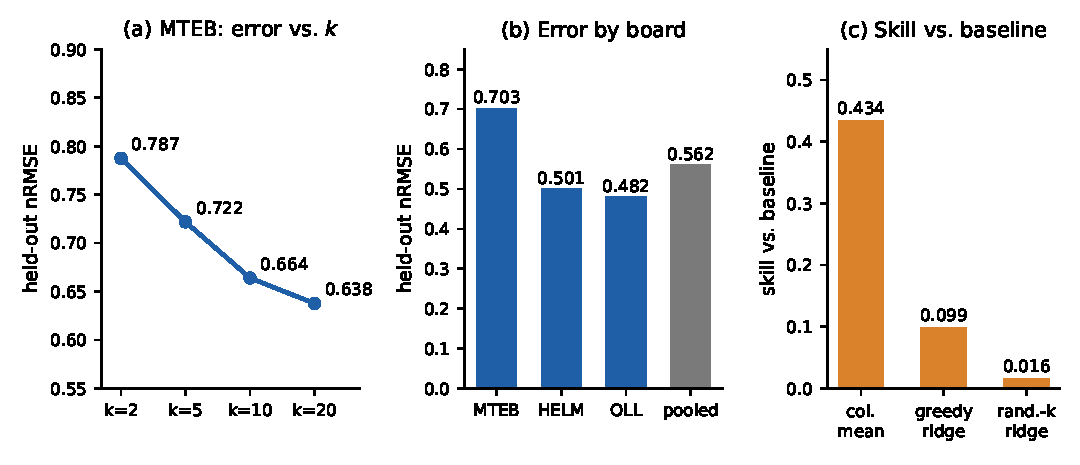
\includegraphics[width=\textwidth]{figures/main_results.pdf}
\caption{Sealed evaluation on family-disjoint held-out models. (a) MTEB $\nrmse$ against budget $k$ (mean over three seeds). (b) $\nrmse$ per leaderboard (OLL: Open LLM Leaderboard) and pooled over the three. (c) Skill against column-mean, greedy-forward ridge and random-$k$ ridge baselines, pooled over leaderboards. No error bars: the retained metrics are seed means, and the three seeds share the same held-out models.}
\label{fig:main}
\end{figure}

\subsection{Main results}
Pooled over the three leaderboards, the evaluated pair reaches $\nrmse=0.562$ and a skill of 0.434 against column-mean imputation, that is, a mean relative error reduction of 43.4\% (Table~\ref{tab:final}). % @evidence[[paper_data.json#final.metric.final_nrmse]] @evidence[[paper_data.json#final.metric.final_score]]
The three per-seed pooled skills are 0.433, 0.427 and 0.433, so the stochasticity of the method's own cross-validation folds moves the headline by less than 0.006. % @evidence[[paper_data.json#final.evidence.episodes]]
This supports H1 in the evaluated setting. Because all three seeds use identical held-out models, this spread does not measure how the result would change with different held-out models, and we report no confidence interval for the pooled values.

\begin{table}[t]
\centering
\caption{Sealed final metrics of the evaluated selector--imputer pair (mean over seeds 201--203; hierarchy described in Section~\ref{sec:protocol}). Lower $\nrmse$ is better; skill is relative error reduction against the named baseline.}
\label{tab:final}
\small
\begin{tabular}{lcl}
\toprule
Metric & Value & Meaning\\
\midrule
Pooled $\nrmse$ & 0.562 & mean over 3 leaderboards\\
\quad MTEB / HELM / Open LLM & 0.703 / 0.501 / 0.482 & per leaderboard\\
\quad MTEB $k{=}2/5/10/20$ & 0.787/0.722/0.664/0.638 & error vs.\ budget\\
Skill vs.\ column mean & 0.434 & H1\\
Skill vs.\ greedy-forward ridge & 0.099 & selector+imputer jointly\\
Skill vs.\ random-$k$ ridge & 0.016 & selector+imputer jointly\\
Permuted-control gap (nRMSE) & 0.678 & control minus real\\
\bottomrule
\end{tabular}
% @evidence[[paper_data.json#final.metric.final_nrmse_mteb]] @evidence[[paper_data.json#final.metric.final_nrmse_helm]] @evidence[[paper_data.json#final.metric.final_nrmse_oll]] @evidence[[paper_data.json#final.metric.final_skill_vs_greedy_ridge]] @evidence[[paper_data.json#final.metric.final_skill_vs_random_selection]] @evidence[[paper_data.json#final.metric.final_permuted_control_gap]]
\end{table}

\subsection{Error against the budget $k$}
On MTEB, $\nrmse$ falls monotonically from 0.787 at $k{=}2$ to 0.722 at $k{=}5$, 0.664 at $k{=}10$ and 0.638 at $k{=}20$ (Figure~\ref{fig:main}a). % @evidence[[paper_data.json#final.metric.final_nrmse_mteb_k2]] @evidence[[paper_data.json#final.metric.final_nrmse_mteb_k5]] @evidence[[paper_data.json#final.metric.final_nrmse_mteb_k10]] @evidence[[paper_data.json#final.metric.final_nrmse_mteb_k20]]
The mean reduction per additional benchmark shrinks from about 0.022 between $k{=}2$ and $5$, to 0.012 between 5 and 10, to 0.003 between 10 and 20 (differences of the four tabulated means divided by the number of added benchmarks). This supports the diminishing-returns part of H2 on MTEB, with four budgets and no uncertainty estimate for each point. Even at $k{=}20$, i.e.\ about 7\% of the 297 columns, the typical per-cell error is still about 0.64 history standard deviations. We cannot say what $k$ is ``enough'': that depends on an error tolerance we did not define, and the curve has no baseline at each $k$ (the retained metrics report baseline skill only pooled over budgets). The curve is measured for one leaderboard; the Open LLM Leaderboard and HELM Lite grids ($k\le3$ of 6 and $k\le5$ of 10) were not retained as per-$k$ curves.

\subsection{Baselines and controls}
\paragraph{Control.} The permuted-observation control raises $\nrmse$ by 0.678 on average over the matched real episodes (Table~\ref{tab:final}). % @evidence[[paper_data.json#final.metric.final_permuted_control_gap]]
Hence the predictions depend on the new model's own scores on the selected benchmarks rather than on a marginal prior alone. The gap is an absolute $\nrmse$ difference and should be read against the pooled error of 0.562.

\paragraph{Selection versus imputation.} Skill against random-$k$ ridge is only 0.016: at the pooled level the proposed pair has a mean relative error 1.6\% lower than five random subsets imputed by a ridge model on a completed history. Skill against greedy-forward ridge is 0.099. % @evidence[[paper_data.json#final.metric.final_skill_vs_random_selection]] @evidence[[paper_data.json#final.metric.final_skill_vs_greedy_ridge]]
Both figures mix selector and imputer, so neither isolates ``which $k$''. The two baselines share an imputer and differ only in selection; since skill against greedy ridge exceeds skill against random-$k$ ridge by 0.083, the averaged skills suggest, but cannot confirm because per-baseline errors were not retained, that the greedy-forward ridge baseline was no better than the random-$k$ ridge baseline. This indicative inference is the only retained evidence about selection alone, and it does not establish that a leave-one-out greedy selector is worse than random subsets under a fixed ridge imputer. For H3 the grounded conclusion is therefore modest. The pair's accuracy over a ridge imputer does not separate into a selector effect and an imputer effect, and the small margin over random-$k$ suggests that on these leaderboards most of the achievable gain over column means is available with a reasonable imputer and an arbitrary subset.

\subsection{Difficulty across leaderboards}
$\nrmse$ is 0.703 on MTEB, 0.501 on HELM Lite and 0.482 on the Open LLM Leaderboard (Figure~\ref{fig:main}b), so H4 holds in the sense that error differs. It is not a clean difficulty ranking: the leaderboards differ in the number of benchmarks (297, 10, 6), history size (124, 66, 3371 models), $k$ grids, and what $k$ means as a fraction of the columns. MTEB lists embedding models over many task types, which is also a different object from generative language models; none of the three results transfers to the others. % @evidence[[analysis/protocol_facts.json#final]]

\subsection{Reading the metrics: sensitivity and failure analysis}
\paragraph{Skill is a mean of ratios.} Each skill value is computed per episode and then averaged along the hierarchy of Section~\ref{sec:protocol}, and is clipped to $[-1,1]$. It is therefore not equal to one minus the ratio of pooled errors. If it were, the two ridge-baseline skills would imply that the greedy-forward baseline has an error about $(1-0.016)/(1-0.099)\approx 1.09$ times that of the random-$k$ baseline. We read this only as indicative of the sign and rough size of the effect. % @evidence[[paper_data.json#final.metric.final_skill_vs_random_selection]] @evidence[[paper_data.json#final.metric.final_skill_vs_greedy_ridge]]
\paragraph{Where the pair could fail.} Three mechanisms can degrade the predictions without being visible in the pooled numbers: (a) benchmarks with few history observations fall back to z-scores or to coarse medians, and the clipped outputs cannot extrapolate beyond the history range, so a new model that outperforms every history model on a benchmark is necessarily under-predicted on that benchmark; (b) selected benchmarks that a new model has not been run on contribute nothing, and the pair then falls back to a prior that conditions on fewer scores (a model with none of the selected scores receives column medians); (c) the wall-clock guards switch off the stack or optional candidates on slow hardware. We did not construct stress tests for (a)--(c), so we cannot report how often or by how much they matter.
\paragraph{What a different outcome would have looked like.} A permuted-control gap near zero would have meant that the predictions were driven by the marginal prior; a negative skill against column means would have refuted H1; a flat MTEB curve would have refuted H2. The first two did not occur and the third is contradicted by the monotone curve, so the study could have refuted them. By contrast, H3 and H4 are not tested sharply: the sealed metrics do not isolate selection, and the leaderboards are not matched in size.

\subsection{Configuration comparison on the model-development partition}\label{sec:search}
During development, three configurations were scored on a separate MTEB partition (disjoint groups, 280 columns, 131 history and 32 held-out models) with two seeds and $k\in\{2,5,10,20\}$. Table~\ref{tab:search} keeps these numbers apart from the sealed ones; $\nrmse$ values are not comparable across the two partitions.
% @evidence[[analysis/search_metrics.json#01]] @evidence[[analysis/search_metrics.json#02]] @evidence[[analysis/search_metrics.json#03]]

\begin{table}[t]
\centering
\caption{Development-partition comparison (MTEB, two seeds). Score is the mean skill against column mean. The seed columns give the two per-seed scores.}
\label{tab:search}
\small
\begin{tabular}{lccccc}
\toprule
Configuration & Score & Seeds 11/12 & $\nrmse$ & vs.\ random-$k$ & Perm.\ gap\\
\midrule
Simple pair (trace + cond.\ mean) & 0.220 & 0.220 / 0.220 & 1.067 & 0.100 & 0.522\\
Proposed pair (wrapper + stack) & 0.247 & 0.243 / 0.251 & 1.028 & 0.132 & 0.568\\
Proposed + latent-skill member & 0.247 & 0.243 / 0.251 & 1.028 & 0.132 & 0.568\\
\bottomrule
\end{tabular}
\end{table}

The proposed pair scores 0.247 against 0.220 for the simple pair, with non-overlapping per-seed ranges (0.243--0.251 vs.\ 0.220), and also shows a larger skill over random-$k$ selection (0.132 vs.\ 0.100). % @evidence[[analysis/search_metrics.json#02]] @evidence[[paper_data.json#result.top_program_01]] @evidence[[paper_data.json#result.top_program_03]]
Because several components change together and the two seeds share one held-out set, this licenses only the statement that the richer configuration was better on that partition; it does not attribute the gain to the transform, the wrapper selector or the stack. The pair extended with a latent-skill member and a latent A-optimal selector produced the same four metrics as the proposed pair to all reported digits. The extension is kept only if it improves cross-validation error, which is consistent with it being inactive, but no diagnostic recording the choice was retained, so the cause is unknown, and we treat this configuration as a null result. The sealed evaluation was run on one of these two configurations; the exact tie means the retained scores cannot say which (Supplementary Information).

\section{Discussion and Limitations}\label{sec:limits}
\paragraph{What is and is not shown.} The sealed result supports a bounded statement: on family-disjoint held-out models from three pinned leaderboards, a history-fitted selector--imputer pair predicts unrun benchmark scores with a mean relative error reduction (skill) of 0.434 against column means, and permuting the observations raises nRMSE by 0.678 on average over the matched real episodes, so the predictions use the new model's own scores. The retained evidence does not report control skill against column means. The evidence does not show that cross-benchmark structure is \emph{exploited by selection}; it shows that observed scores help, and that a random subset with a ridge imputer comes within a skill of 0.016 of the pair.

\paragraph{Joint scoring and missing ablations.} Selector and imputer are scored together. No controlled experiment varied one while holding the other fixed, so the contributions of the rank-Gauss transform, the wrapper selector, the stack and the clipping are unattributed. The development-partition comparison changes many components at once. A fair selector test would pair each selector with each imputer; we did not run it.

\paragraph{Uncertainty.} Reported values are seed means. The seeds vary only the method's internal randomness (fold assignments), not the held-out models, baselines or controls, so the 0.006 spread across seeds understates sampling uncertainty over models. Held-out sets are small for MTEB (37 models) and HELM Lite (25), and the held-out groups are few (25 and 7). The 0.016 margin over random-$k$ should be viewed as indistinguishable from zero until a resampling-based interval over held-out models is available; we did not compute one, and we make no significance claim.

\paragraph{Scope.} Three leaderboards, of which two contain generative language models in small numbers of benchmarks (six and ten) and one contains text-embedding models; metric types differ (accuracy-type, F1, exact-match and BLEU-type metrics). Family-disjoint splitting was defined by name and content heuristics. Selection is non-adaptive; adaptive stopping or sequential selection could change the picture. If leaderboard missingness correlates with model strength, the missing-at-random assumption of EM-based imputation \citep{Rubin1976Inference} may fail; we did not test this. The run-time guards in Section~\ref{sec:impl} make behaviour hardware-dependent.

\paragraph{Unperformed analyses.} We did not run a theory check of the trace objective, a component ablation, per-family error breakdowns, comparisons with low-rank matrix completion or latent-factor imputers as full alternatives, or other leaderboards. These are not claimed.

\paragraph{Threats to validity.} (1) \emph{Leakage through naming.} Family-disjointness relies on name normalisation, a family key and a content hash; a model re-released under an unrecognised name could cross the split. (2) \emph{Metric scale.} Errors are in history standard deviations of each benchmark, which makes a benchmark with a narrow history spread (e.g.\ one saturated by strong models) look harder to predict than one with a wide spread. (3) \emph{Heterogeneous coverage.} If leaderboard missingness depends on model strength or recency, benchmarks selected for a new model may be sparsely covered in the history; we did not analyse missingness. (4) \emph{Configuration identity and freezing.} The configuration was chosen on the development partition before the sealed evaluation, but no artifact records which of the two tied configurations the sealed run used or that it was run only once, and the identity of the sealed-evaluated tree is not established; the sealed numbers are not selected on, but the development partition is from the same MTEB snapshot, so the MTEB result is closer to the development distribution than the other two leaderboards, which were not used to choose among configurations. (5) \emph{Implementation coupling.} The result is for one concrete implementation, including its tuning grids and wall-clock guards; a different implementation of the same design could behave differently.

\paragraph{Practical reading.} In these experiments, with the evaluated pair, a few benchmark runs already reduced the column-mean error (pooled skill 0.434), additional benchmarks on MTEB bought progressively less, and a residual error of about 0.64 history standard deviations remains for the evaluated pair on MTEB at $k{=}20$, with no claim about a lower bound.

\section{Conclusion}
We posed the cold-start question of how well $k$ benchmark runs predict the remaining scores of a model from an unseen family, and evaluated a rank-Gauss, EM-Gaussian, wrapper-selected, NNLS-stacked selector--imputer family (the exact evaluated source tree is not established by the retained artifacts) on three leaderboards with family-disjoint held-out models. The sealed evaluation completed and qualified. Pooled nRMSE is 0.562 and skill against column means is 0.434, with a clear gap to permuted controls; on MTEB the error decreases from 0.787 to 0.638 as $k$ rises from 2 to 20 with sharply diminishing returns, and error levels differ across leaderboards. The margin over random-$k$ selection with a ridge imputer is only 0.016 and cannot be assigned to selection or imputation, and the averaged skills only suggest, without per-baseline errors to confirm, that a leave-one-out greedy ridge baseline was no better than random subsets. The main unresolved questions are the isolated value of selection, uncertainty over held-out models, and behaviour beyond these three leaderboards; each needs additional controlled experiments that this study did not perform.

\clearpage
\bibliography{references}
\bibliographystyle{paper}

\clearpage
\appendix
\section{Supplementary Information}

\subsection{Evaluation protocol details}
Table~\ref{tab:data} lists the data partitions used by the sealed evaluation, taken from the evaluator's dataset manifests. % @evidence[[analysis/protocol_facts.json#final]] @evidence[[scripts/extract_protocol_facts.py]]
Group counts are numbers of family groups after union-find merging. The model-development partition (MTEB, 280 columns, 131 history models, 32 held-out models, revision identical to the sealed MTEB revision) uses a disjoint set of groups. % @evidence[[analysis/protocol_facts.json#search]]

\begin{table}[h]
\centering
\caption{Sealed evaluation partitions.}
\label{tab:data}
\small
\setlength{\tabcolsep}{4pt}
\begin{tabular}{lcccccc}
\toprule
Leaderboard & Revision & Cols. & History & Held-out & Groups (h/o) & $k$ grid\\
\midrule
MTEB results & 6dabbcc & 297 & 124 & 37 & 92 / 25 & 2, 5, 10, 20\\
Open LLM Leaderboard & 9c09a7c & 6 & 3371 & 300 & 2314 / 266 & 1, 2, 3\\
HELM Lite & v1.13.0 & 10 & 66 & 25 & 16 / 7 & 2, 3, 5\\
\bottomrule
\end{tabular}
\end{table}

\noindent Score definitions: MTEB uses each task's main score averaged over the entries of the first available split (test, validation, dev, train), taken from the model revision directory with the most task files; Open LLM Leaderboard uses raw scores of IFEval, BBH, MATH Level 5, GPQA, MUSR and MMLU-PRO, dropping rows with a missing score; HELM Lite uses the ten scenario columns of the core-scenarios table, excluding the mean-win-rate column. Held-out MTEB and HELM Lite models may lack some scores; those cells are not scored. Per-seed pooled scores of the sealed evaluation were 0.4330 (seed 201), 0.4273 (202) and 0.4328 (203), taking 157.4, 160.6 and 161.0 seconds for 14 episodes each. % @evidence[[paper_data.json#final.evidence.episodes]]

\subsection{Method specification and hyperparameters}
Table~\ref{tab:hyper} collects the constants of the pair described in Section~\ref{sec:impl}; they are read from the entry-point source of the proposed-pair source copy (\texttt{src/program.py}: the EM, greedy-selection, wrapper-selection, stacking and prediction routines). This copy is not verified to be the exact tree evaluated in the sealed run (see below), so the constants describe the proposed pair, not a confirmed record of the sealed configuration. % @evidence[[source_evidence/config_proposed/program.py]]

\begin{table}[h]
\centering
\caption{Constants of the proposed pair, read from its source copy (not verified as the exact sealed-evaluated tree).}
\label{tab:hyper}
\small
\begin{tabular}{lp{0.5\textwidth}}
\toprule
Component & Setting\\
\midrule
EM & shrinkage 0.02, $\le 60$ iterations, tol.\ $10^{-4}$, jitter $10^{-4}$, 25-s budget\\
Cross-validation & 5 folds over history models\\
Covariance shrinkage grid & 0, 0.05, 0.15, 0.3\\
Factor-rank grid & 2, 4, 6, 10, full\\
Ridge $\lambda$ grid (Gaussian conditional mean) & 0.003, 0.03, 0.1, 0.3\\
Selection candidates & 4 trace-greedy settings, 2 wrapper settings (coverage exponent 0 or 1)\\
Wrapper & $\lambda=0.1$, shrinkage 0.05, $\le 250$ candidates per step\\
Stack base predictors & Gaussian conditional means (shrink 0, 0.15, 0.3), ridge ($\lambda=5$), kNN (5, 15)\\
Stack regularisation grid & 0, 0.05, 0.25, 1, 5, $10^{5}$\\
Clipping & z-scores at $\pm 8$; outputs to the history range\\
Wall-clock guards & skip optional candidates 70 s; smaller tuning grid 150 s; skip stacking 210 s\\
\bottomrule
\end{tabular}
\end{table}

\noindent The latent-skill extension (third row of Table~\ref{tab:search}) adds a low-rank model $T_{ij}\approx g_j(u_i\cdot v_j+b_j)$ with a monotone piecewise-linear link $g_j$ per benchmark, Huber-likelihood MAP inference of a new model's latent vector with a Laplace covariance, an additional stack member retained only if cross-validation improves, and a latent A-optimal selector candidate. Its metrics equal those of the proposed pair (Table~\ref{tab:search}); the extension took roughly 331--334 seconds per search seed against 141--142 seconds for the proposed pair. % @evidence[[analysis/search_metrics.json#03]]
The longer run time indicates that the extra code ran, but its influence on outputs is not established. The final-evaluation record lists a hash of the evaluated source tree; no hash-comparison artifact is available, so the identity of the evaluated tree is not established, and the tie above means the retained scores cannot discriminate the two. The main text describes the shared stack, and the extension is described here because the sealed run may have used it. The simple pair used 95--97 seconds per search seed. % @evidence[[analysis/search_metrics.json#01]]

\subsection{Extra evidence tables}
\begin{table}[h]
\centering
\caption{Development-partition per-seed scores and durations (seconds, two seeds each).}
\label{tab:seeds}
\small
\begin{tabular}{lcccc}
\toprule
Configuration & Score (seed 11) & Score (seed 12) & Time (seed 11) & Time (seed 12)\\
\midrule
Simple pair & 0.2201 & 0.2197 & 95.4 & 97.3\\
Proposed pair & 0.2429 & 0.2506 & 140.9 & 142.2\\
Proposed + latent member & 0.2429 & 0.2506 & 331.2 & 334.3\\
\bottomrule
\end{tabular}
% @evidence[[analysis/search_metrics.json]]
\end{table}

\subsection{Unperformed analyses}
The following were not run and are not claimed: component ablations (the ablation directory of the run is missing); empirical verification of the trace objective as expected error; bootstrap or model-resampling intervals; per-leaderboard $k$ curves for Open LLM Leaderboard and HELM Lite as retained metrics; baseline $\nrmse$ values per budget; additional leaderboards such as LiveBench, BigCodeBench or AlpacaEval, which the task description lists as optional.

\subsection{Reproducibility and data sources}
Entry point: a single Python file exposing a \texttt{handle} request function (operations \texttt{reset}, \texttt{load\_history}, \texttt{select}, \texttt{predict}); dependencies are NumPy only; behaviour is deterministic given the seed except for the wall-clock guards. Figures and tables in this paper come from \texttt{scripts/build\_figures.py} (Figure~\ref{fig:main}), \texttt{scripts/extract\_protocol\_facts.py} (Table~\ref{tab:data}), \texttt{scripts/extract\_search\_metrics.py} (Tables~\ref{tab:search} and~\ref{tab:seeds}); the sealed metrics are read from the evaluation registry. The data come from the public upstream sources and pinned revisions listed in Table~\ref{tab:data}; licence terms of these sources were not verified in this study. Literature retrieval used only titles from the starter literature and standard methodology references; no material from the excluded publication was knowingly accessed.

\subsection{LLM Usage}
Large language models were used for research hypothesis generation, for implementing and running the compared configurations, and for drafting and editing this manuscript. The selector--imputer designs, code, experiments and the text were produced by an automated LLM-driven research workflow, with evaluator-owned scoring that the workflow could not modify. All reported numbers were read from evaluator outputs and checked against the evidence registry; the human role was limited to specifying the task and evaluation setting. References were retrieved from bibliographic databases and checked against their records.

\end{document}
